\chapter{Расчетная модель}
\label{Chapter2}
\setlength{\parindent}{0pt}

\section{Описание}
Для расчета изменений давления в приструйной зоне во времени примем расчетный цикл. На каждой его итерации будем рассчитывать величину потерь на эжекцию воздуха и вычитать её из текущего значения давления. Тем самым будет получено новое значение давления в приструйной зоне, которое будет использовано в следующей итерации как текущее. Изменящееся внешние давление будет оказывать влияние на режим истечения струи и её эжектирующую способность, что также повлечет за собой изменение величины потерь.

\section{Основные соотношения}
Основным расчетным соотношением является формула 

\begin{equation}
    \label{eqn:MainPressure}
    P_\text{п}=P_\text{в}-h_\text{э}-h_\text{м},
\end{equation}

в которой отражены потери полного давления на эжекцию воздуха и потери давления на местных сопротивлениях. Полное давление приравнено к окружающему. Потери на эжекцию определяеются следующим соотношением

\begin{equation}
    \label{eqn:EjectionLosses}
    h_\text{э}=\dfrac{\rho\upsilon_\text{э}^2}{2}.
\end{equation}

Потери на потери давления на местных сопротивлениях определяются в соответствие с расчетной схемой, изображенной на \hyperref[fig:LossesScheme]{рисунке 2.2.1}

\begin{figure}[H]
    \label{fig:LossesScheme}
    \centering
    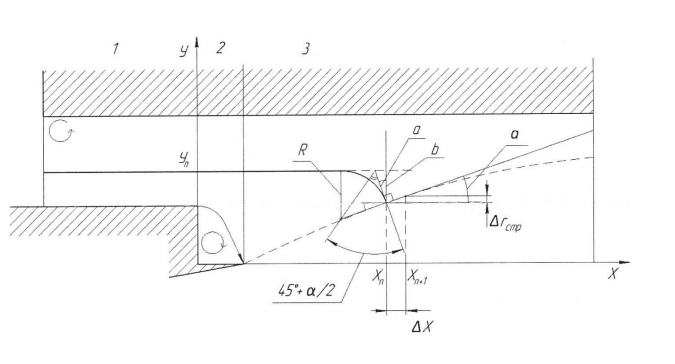
\includegraphics[height=6cm]{Figures/Scheme.png}
    \caption{Схема расчета потерь на местных споротивлениях}
\end{figure}

По схеме, эти потери выражаются в трех составляющих - потерях на внезапное сужение канала, на участке 1, потерях на внезапное расширение канала, на участке 2, и поворот канала, на участке 3. Соответственно, имеем формулу

\begin{equation}
    \label{eqn:LocalLosses}
    h_\text{м}=h_\text{с}+h_\text{р}+h_\text{п}.
\end{equation}

Таким образом, имея ввиду расчетные соотношения \hyperref[eqn:EjectionLosses]{2.2.2}, \hyperref[eqn:LocalLosses]{2.2.3}, требуется определить зависимости потерь от параметров течения струи.

\section{Потери на эжекцию}
В соответствии с \hyperref[eqn:EjectionLosses]{формулой 2.2.2} для определения потерь на эжектирующем участке струи необходимо определить скорость эжектируемого потока для каждого сечения. Для этого воспользуемся соотношением

\begin{equation}
    \label{eqn:EjectionVelocity}
    \upsilon_\text{э}=\dfrac{C_\text{ст}}{2\pi\rho r_\text{ст}}.
\end{equation}

Величина $C_\text{ст}$ - эжекционная способность струи, принимается постоянной по её длине. Для определения введем формулу

\begin{equation}
    \label{eqn:EjectionAbility}
    C_\text{ст}=\dfrac{Q_\text{зв}-m}{x_\text{зв}}.
\end{equation}

Формула для расхода

\begin{equation}
    \label{eqn:Consumption}
    m=\varphi(\dfrac{F_\text{кр}BP_{0}}{\sqrt{RT}}),
\end{equation}

где $F_\text{кр}$ - площадь критического сечения сопла, определяемая как

\begin{equation}
    \label{eqn:CriticalSquare}
    F_\text{кр}=\dfrac{F_\text{а}}{\dfrac{1}{M^2}((\dfrac{2}{\gamma+1})(1+M^2 \dfrac{\gamma-1}{2}))^{\dfrac{\gamma+1}{\gamma-1}}},
\end{equation}

a также $B$ и $\varphi$, коэффициенты потерь в сопле Лаваля,

\begin{equation}
    \label{eqn:LavalKoef2}
    B=(\dfrac{2}{\gamma+1})^{\dfrac{\gamma+1}{2(\gamma-1)}},
\end{equation}

\begin{equation}
    \label{eqn:LavalKoef1}
    \varphi=0.98,
\end{equation}

и начальное давление в камере сгорания

\begin{equation}
    \label{eqn:StartPressure}
    P_\text{0}=P_\text{а}(1+\dfrac{\gamma-1}{2} M^2)^{\dfrac{\gamma}{\gamma-1}}.
\end{equation}

Величины $Q_\text{зв}$ и $x_\text{зв}$ характеризуют звуковое сечение - такое, в котором скорость истечения газа равно скорости звука. Сначала определяется координата сечения на оси струи

\begin{equation}
    \label{eqn:SonicCoord}
    x_\text{зв}=(13.28 \sqrt{\gamma M^2} + 11.8) \sqrt[3]{\eta}-23.57.
\end{equation}

Затем, по данным рассчета геометрии струи определяется радиус этого сечения. С его помощью определяем расход через звуковое сечение

\begin{equation}
    \label{eqn:SonicConsumption}
    Q_\text{зв}=0.217 \pi l r_\text{ст.зв}^2,
\end{equation}

где, соответственно

\begin{equation}
    \label{eqn:SonicVelocity}
    l=\sqrt{\dfrac{\gamma}{RT}} P_\text{в} \sqrt{\dfrac{\gamma+1}{2}}.
\end{equation}

Таким образом, имеем все необходимые соотношения для определения величины потерь на эжекцию воздуха по \hyperref[eqn:EjectionLosses]{формуле 2.2.2}.

\section{Потери на местных сопротивлениях}
Из \hyperref[eqn:LocalLosses]{формулы местных потерь 2.2.3} имеем потери при внезапном сужении канала, выраженные формулой

\begin{equation}
    \label{eqn:ConstrictionLosses}
    h_\text{с}=\zeta_\text{с} \dfrac{\upsilon_{12}^2}{2g},
\end{equation}

потери при внезапном расширении канала, выраженные формулой

\begin{equation}
    \label{eqn:ExpansionLosses}
    h_\text{рв}=\zeta_\text{р} \dfrac{\upsilon_{23}^2}{2g},
\end{equation}

и, потери при повороте, выраженные формулой

\begin{equation}
    \label{eqn:RotationLosses}
    h_\text{рв}=\zeta_\text{п} \dfrac{\upsilon_{23\text{ср}}^2}{2g}.
\end{equation}

Коэффициент потерь при внезапном сужении постоянен и равен

\begin{equation}
    \label{eqn:ConstrictionLossesCoef}
    \zeta_\text{с} = 0.5
\end{equation}

потерь при внезапном расширении определяется перепадом сечений и равен

\begin{equation}
    \label{eqn:ExpansionLossesCoef}
    \zeta_\text{р}=(1-\dfrac{S_{2}}{S_{3}})^2.
\end{equation}

Коэффициент потерь при повороте канала определяется углом поворота

\begin{equation}
    \label{eqn:RotationLossesCoef}
    \zeta_\text{п}=0.95 (\sin(\dfrac{\alpha}{2}))^2 + 2.05(\sin(\dfrac{\alpha}{2}))^4.
\end{equation}

Для определения этого угла используем схему на \hyperref[fig:LossesScheme]{рис. 2.2.1}.
По длине струи делим её на конечные участки и определяем на этих учатсках разницу в радиусе границы.
После чего, определяем угол через арктангенс

\begin{equation}
    \label{eqn:RotationLossesCoef}
    \alpha= \arctan (\dfrac{\varDelta r_\text{ст}}{\varDelta x_\text{ст}}).
\end{equation}

Скорости газа на всех учатсках определяются из закона постоянства расхода.

